\documentclass{acm_proc_article-sp}

\usepackage{graphicx}

\begin{document}

\title{Determining Community Interest in\\Text-Only Posts on Reddit}
\subtitle{Project Proposal}

%
% You need the command \numberofauthors to handle the 'placement
% and alignment' of the authors beneath the title.
%
% For aesthetic reasons, we recommend 'three authors at a time'
% i.e. three 'name/affiliation blocks' be placed beneath the title.
%

\numberofauthors{3}

\author{
% You can go ahead and credit any number of authors here,
% e.g. one 'row of three' or two rows (consisting of one row of three
% and a second row of one, two or three).
%
% The command \alignauthor (no curly braces needed) should
% precede each author name, affiliation/snail-mail address and
% e-mail address. Additionally, tag each line of
% affiliation/address with \affaddr, and tag the
% e-mail address with \email.
%
% 1st. author
\alignauthor
Charles Lewis\\
       \affaddr{University of Michigan}\\
       \affaddr{Ann Arbor, MI}\\
       \email{noodle@umich.edu}
% 2nd. author
\alignauthor
Nathaniel Price\\
       \affaddr{University of Michigan}\\
       \affaddr{Ann Arbor, MI}\\
       \email{nrprice@umich.edu}
% 3rd. author
\alignauthor
David Purser\\
       \affaddr{University of Michigan}\\
       \affaddr{Ann Arbor, MI}\\
       \email{dpurser@umich.edu}
}

\date{21 April 2014}

\maketitle
\begin{abstract}
This paper proposes a term project for the EECS 498 Information Retrieval
course at the University of Michigan which seeks to analyze content on 
Reddit\footnote{\texttt{http://www.reddit.com/}} to determine community
interest in certain topics, keywords, and questions.

The project involves collecting a set of data from a number of subreddits
(individual forums on Reddit) including textual content of each post,
number of votes that the post received, number of comments on the post, and
other information.  This information will be used to estimate the community's
interest in each post.  These estimates will be compiled and indexed by keyword,
allowing a user to query the system to determine the expected interest in a
new post and whether a new post is very similar to previous posts.
\end{abstract}

% A category with the (minimum) three required fields
\category{H.3.1}{Information Storage and Retrieval}{Content Analysis and Indexing}
\category{H.3.3}{Information Storage and Retrieval}{Information Search and Retrieval}
%A category including the fourth, optional field follows...
%\category{D.2.8}{Software Engineering}{Metrics}[complexity measures, performance measures]

%\terms{Algorithms, }

\keywords{Data analysis, Reddit, community interest} % NOT required for Proceedings

\section{Problem}
We sought to explore whether it was possible to predict whether a post would be popular (community interest) or not on \texttt{www.reddit.com}, specifically text-only posts on subreddits sucht as \texttt{/r/AskReddit} or \texttt{/r/ELI5}. \texttt{Reddit} is a platform where users upvote and downvote posts based on various criteria. The users also have the option of posting a comment on a particular post. The overall motivation was to research different machine learning and information retrieval process in order to figure out which would prove to be helpful in determining community interest on \texttt{Reddit}.

There are various applicaitons in which this work would benefit. This could help indicate when it might be a useful time to repost something. The community of Reddit has a strong aversion to things that are posted often. These are often refered to ``reposts''. However, there is some benefit to reposts. Users that are recently new will find the content new and relevant to them. In addition, there is benefits to bringing up a topic again as it will generate close to the same community interest as it did when it was initially posted. Our work could provide a way of detecting when might be the best possible time to repost something for it to be meaningful and relevant to the community.

An alternative application could be for buisness marketting. Knowing how a particular community will respond to your post can help buisness tailor their marketing strategies to a particular subreddit. There is also the possibility that future work on some of the proposed solutions/methods that we researched could help indicate things that a marketer could change in order to make their content generate more interest.

\section{Previous Work}
<NEED TO ADD TO THIS>

There are a number of websites dedicated to detecting ``reposts'' on Reddit, which are
exact duplicates of previously posted content.  One such website is KarmaDecay\footnote{\texttt{http://karmadecay.com/}}.
However, these websites only detect exact duplicates of hyperlinks and images, which make
up the majority of posts in many subreddits.  The textual content of posts in text-only
subreddits such as \texttt{/r/AskReddit} or \texttt{/r/ELI5} is not analyzed.
This gives these websites limited usefulness in text-only subreddits, where no images or external
links are generally allowed.

Furthermore, existing systems are designed mostly to help users avoid reposting exact duplicates of
existing material, and do not match based on a similarity measure.  This means that related or
very similar posts will not be matched, only exactly identical ones.  By using a text-matching system based
on similarity scores,
our project will allow text-only topics to be analyzed not to detect exact duplicates (as these
are rare in text posts due to the diversity inherently present in language), but to find similar
posts from the past based on matching keywords, topics, phrases, and other
content.  These similar posts can then be used to judge or estimate potential interest in the new
post and to predict useful information such as whether a post will be popular or successful or
which subreddits it may be most successful in by analyzing the interest in the previous posts. 
In addition, the uniqness of the post will also contribute to determing how popular a post might be.

Therre has been work done analyzing news content, not based on the article but
upon the responses of the general public \cite{liu:interest}. This paper describes
a way of what they describe as ``comment centric tagging'' as a means to identify
which articles were highly interesting and important. They use these comments within
a post to alter and adapt the interest weighting on an article. 

While this work is not the main focus of the paper, it does highlight how important
the comments of a post can be. The study they performed showed that the comments 
of a post greatly impacted the community interest within that specific topic. This will
help us direct or findings towards the comments found on Reddit, weighing them higher,
than the actual post itself.

Some work has also been done by researchers to determine characteristics of articles that
have been ranked by crowdsourced feedback from users \cite{askalidis:crowdsourced}.
The results of this study point out that while crowdsourced feedback mechanisms ``can be
relatively effective for \ldots promoting content of high quality, they do not perform well
for ordinal objectives such as finding the best articles.''  In other words, while interesting
topics and general themes are often highlighted as outstanding by user feedback, the best
specific articles are not always at the very top of the list.  Rankings which are based on
user feedback will likely tend to positively identify good
topics, but perhaps not the absolute best topics.  This means that we should not use a post's
score as an absolute ranking; that is, we should not conclude that one post is definitively better
than another simply because it has a higher score.  For our purposes, this means that
all posts with a reasonably high score could be determined to be interesting to the
community, but that comparing levels of interest (or ranking the level of interest)
between two interesting topics will likely be very difficult.

The article also has some
interesting discussion about crowdsourced scores over time, indicating that posts tend
to take a while to gain momentum, but then explode rapidly if they are determined to
be interesting.  This means that some posts which are not ``discovered'' by users (they
may be posted at the wrong time of day or when few users are online, so they are not
identified by interested users) may fail to gain traction and perform as they should.
This may mean that the same post, created at different times, may be extremely popular
one time and not at all another time.  In fact, the post may go unnoticed several times
and only be discovered once.  Our scoring algorithms will have to take this
into account, likely by giving the positive feedback of posts which are determined to
be interesting much more weight than the negative feedback of posts which are determined
to be uninteresting (because a post that scores highly is almost certainly
an indicator of community interest, while a post that scores poorly may have many
different reasons for receiving that score).

Work has been done in this area before by another Michigan student, targeting
Digg instead of Reddit. His
website\footnote{http://gigaom.com/2010/08/24/hey-digg-this-17-year-old-knows-what-you-are-thinking/}
analyzed all of the most recently-posted links on Digg, and used various
heuristics to predict which articles would make it to the front page. Various
differences between the algorithms used by the two sites make it impossible to
use the exact same approach here--the code relied on being able to see which
users voted on which articles, while on Reddit this information is made private
by default. In addition, Digg weighted the votes of some users above others
instead of treating everyone equally. The fundamental concept of extrapolating
early votes to predict eventual popularity will still be an important concept
for us to investigate.

In addition to using upvotes and downvotes to rank content, reddit keeps track
of the total score of all of a user's comments. Power users of reddit have a
strong incentive to identify posts that will eventually reach the front page,
since commenting early on these threads provides the maximum return of points
for the time spent. To this end, the subreddit \texttt{/r/risingthreads} tries
to identify these threads within minutes of when they are posted, but how it
does this is not known. The submissions to this subreddit are submitted by a
bot, that presumably flags posts with lots of early upvotes. In the sidebar of
the subreddit, \texttt{/r/askreddit} is specifically named as a subreddit for
which the bot's algorithm performs poorly. Our project, by analyzing the text
content of the post and its comments, may be able to improve upon this
performance. This subreddit also shows a way to get user feedback on our
project's effectiveness. If our project works well enough, we could set up our
own subreddit to share and test its results.

\section{Approach}
Our approach for this project involves three major areas: data collection, processing, and retrieval.

First, data must be collected from Reddit.  This will involve collecting and indexing a number of past posts
in text-only subreddits.  The posts and their comments will be analyzed, looking for common keywords,
themes, or topics which seem relevant to the post in order to match the post with other submissions
that have similar topics.

We focused on the upvotes of a redit post. When implementing our various different systems, we focused on the score as our measure of community interest. We thought of using the comments instead of the score, or inconjunction with the score, but we did not experiment and analyze that within our research and implementations.

There were three different implementations that we approached: cosine similarity between topics, naive bayseian on the words found within the posts, and a boolean classifier machine learning approach. We believed that each method had benefits and disadvantages and wanted to experiment with the various different methods to see which method, if any, peformed better than the baseline.

\subsection{Cosine similarity-weighted scoring}

The premise of this method is our expectation that the scores of new submissions will correspond approximately
with the scores of past submissions that are very similar, which we can judge by the similarity of their titles.
All of the indexed submissions are therefore tokenized with a regular-expression based tokenizer that
separates words, and then passed through a standard Porter stemmer\footnote{http://tartarus.org/~martin/PorterStemmer/}.
Once tokenized and stemmed, the tokens are placed into an index using the tfc-nfx\cite{salton} algorithm.

To determine the expected score of a submission, the index is then queried using the tokens from the new submission's
title, matching by cosine-similarity.  For this method, the ``score'' of each similar topic is calculated using the formula
$upvotes - downvotes + comments*2.5$, where $comments$ represents the number of comments that the post received.  The values
used were all takes after the post had existed for one full day.

Other methods of scoring were also tested, including only using upvotes, or only number of comments.  The stated method of
scoring appears to work best for this algorithm, although some others produced similar results.  The score returned is not
intended to correspond with any score available from Reddit or any other source; it is an arbitrary number only comparable to
other scores returned by the algorithm.

A weighted average was then taken of the scores of each post returned by the index, using the square of the cosine-similarity
result.  The similarity is squared to minimize the effects of the ``long tail'' of posts that have relatively low similarity, but which
would otherwise dominate the average because of their large quantity.

By analyzing the posts returned from the index, we can see that this method does fairly accurately recognize similar
and related questions as we would expect, since it works very much like a search engine looking through old posts.  However, the
method has a number of downsides that would prevent it from working properly under certain conditions.

First, questions which contain unique words and tokens will match fewer submissions from the index, despite the fact that they are probably more
interesting than the average question because of their uniqueness.  This will result in a lower score being predicted for those
posts, which will lead to lower accuracy for these types of posts.

Second, questions which contain many common words will likely match other submissions with very common words, and therefore their
scores will be lowered.  The use of the tfc-nfx algorithm reduces the effect of this by decreasing the weight of the common words, but
for a question whose title consists \emph{only} of common words, tfc-nfx will not be able to correctly match similar posts.

Because some words appear on AskReddit with fairly high frequency, such as the words ``Reddit'' and ``Redditors'', a stopword eliminator
was implemented and these words were added to the filter.  This further reduces the impact of this problem, but also leads to an increased
occurrence of the third problem: posts which do not match any previously existing posts cannot be scored at all.  This could happen
because the post contains only unique words (words that do not appear in any other submissions) after stopword removal.

<keyword approach>

<machine learning approach>
Next, the popularity or interest of the post will then be measured through various statistics including
number of comments, number of upvotes/downvotes received (through Reddit's voting system), number
of distinct users who commented on the post, average length of the comments, average depth of
comment trees\footnote{On Reddit, users can comment on other comments, forming a tree-like structure of comments.},
number of upvotes/downvotes on comments and their distribution among the comments, time of day that the post was made,
and how long the post has been on Reddit.\footnote{Reddit's algorithm works in such a way that posts that have been on Reddit
a long period of time have a lower ``score''. We may have to inflate the score given to older posts as their ranking
has decayed over time.}

Finally, the keywords, and posts matching those keywords, will then be used to create a database which
can be used to judge popularity of a post based on which keywords appear in the post title or text
body.  This database can then be queried to determine expected popularity of a new post given its
text.  This database will also be designed in such a way that new posts on Reddit will be automatically
incoporated into the corpus.
The query system may also be able to suggest similar keywords (words which are frequently used with
the ones in the given text), topics, or information to include in the post which may increase
the post's popularity score (and thus hopefully lead to a more interesting post on Reddit).
\footnote{This is a possible extension of the project and will need to be explored further.}

\section{Evaluation}
Initially, we experimentally determined what would a good threshold be to determine whether something was popular or not (whether it generated sufficient community interest). To do this, we randomly sampled the data five different times to look for correlations in the posts. We looked at the spread of posts to help figure out what our threshold should be. The graphic below shows this data from a random 240 posts. For the purposes of our evaluation, we determined that a score of 20 or above would be deemed as popular by the community, and anything less than that would be unpopular. \footnote{20 or above represents the top 5\% of Reddit posts}

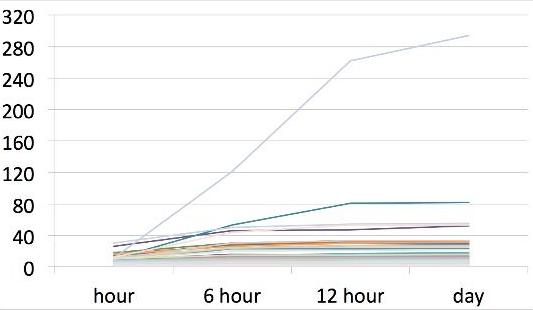
\includegraphics[width=8cm]{evaluation.jpg}\\
(random sample of 240 posts. y-axis = score, x-axis is time)

We initially used a data set cultivated from a week of posts. This data set included 20,000 posts to \texttt{/r/AskReddit} but was later cut down to 17000 posts once all the deleted posts were removed (by the user or by a moderator). This dataset consisted largely of posts that did not make it to the front page and we not seen by users. These post generated little to no community interest. Out of the 17000 posts, about 270 generated community interest. We initially supplied each implementation with this dataset for training and evaluation.

We built an additional, balanced data set as well. This dataset contains an equal amount of popular versus unpopular posts. This dataset was used to make sure that there was no bias in the data that was skewiing our results. This dataset contains 1,977 posts above a 20 upvote threshold and 1,977 below a 20 upvote threshold.

We additionally built a third dataset to that incorporates the balanced dataset with a time weighting. Time of day plays a major factor into whether a post will be successful or not on Reddit. We wanted to utilize a dataset that helps incooperate this time factor into account. 

To generate this dataset, we counted the number of submissions that scored above the threshold of 20 upvotes in each two-hour period
(based on the submission's creation time).  The average number of submissions above the thershold in each two-hour period was 164.75.
For each of the two-hour periods, the actual number of threshold-reaching submissions in that period was divided by the average to
determine a ratio, which roughly corresponds to how well submissions in that two-hour period are expected to perform.  The results
of this process can be seen in the table below.

\begin{table}[h!]
    \begin{tabular}{l|llll}
    Time  &             & Above   &      &       \\
    (UTC) & Submissions & Thresh. & \%   & Mult. \\ \hline
    0:00-2:00        & 3762        & 139             & 3.69 & 1.19       \\
    2:00-4:00        & 3796        & 153             & 4.03 & 1.08       \\
    4:00-6:00        & 3544        & 122             & 3.44 & 1.35       \\
    6:00-8:00        & 2526        & 85              & 3.37 & 1.94       \\
    8:00-10:00       & 1927        & 102             & 5.29 & 1.62       \\
    10:00-12:00      & 2155        & 181             & 8.40 & 0.91       \\
    12:00-14:00      & 3145        & 225             & 7.15 & 0.73       \\
    14:00-16:00      & 3880        & 224             & 5.77 & 0.74       \\
    16:00-18:00      & 3862        & 200             & 5.18 & 0.82       \\
    18:00-20:00      & 3823        & 219             & 5.73 & 0.75       \\
    20:00-22:00      & 3804        & 176             & 4.63 & 0.94       \\
    22:00-0:00       & 3640        & 151             & 4.15 & 1.09       \\
    \end{tabular}
\end{table}

\begin{figure}[h!]
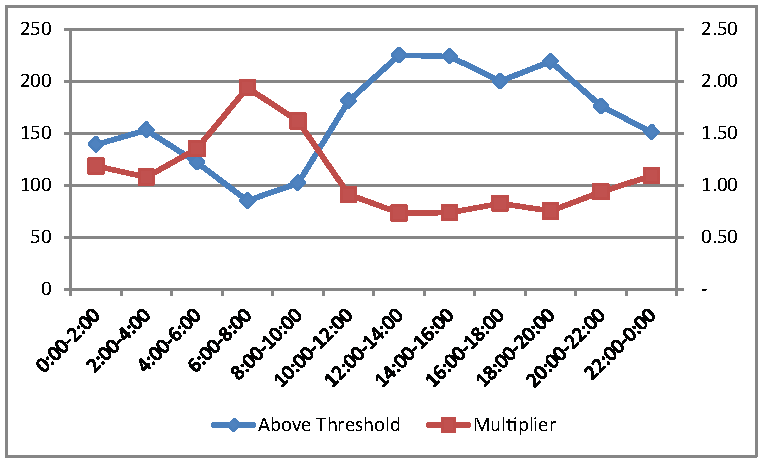
\includegraphics[width=8cm]{timeweightinggraph.pdf}
\end{figure}

Once the ratios were determined, each submission's scores were divided by the ratio (multiplied by the reciprocal, which is shown in the
table) for their creation time period.  That is, posts between midnight and 2:00 AM UTC had their scores multiplied by 1.19, because they
tended to perform slightly worse than average.

This has the result of scaling up the scores of posts made during off-peak hours, and scaling down the scores of posts made during peak
hours, so that by using the scaled scores, posts have a more-or-less even score distribution throughout the day.

When evaluating the systems with each dataset, we tested on how well it worked on a subset of that dataset. For example, we might use 80\% of a given dataset as training and the reamining portion of the dataset for testing. We would go through and mark posts as being popular or unpopular based on our threshold. Then, we would use each of our implementations to go through the dataset and classify the posts. We would then compare how the specific implementation did by using the formula $\frac{Number Classified Correctly}{Total Classified}$. This would give us a percentage how well it classified the posts.

In all of the implementations we compared against marking every post as unpopular. Over 95\% of the posts on Reddit are unpopular, so for our systems to be successful we had to achive better than marking everything as unpopular. 

\section{Results}

<keyword approach>

\subsection{Cosine similarity-weighted scoring}

Unlike the other two implementations, the cosine similarity-weighted scoring algorithm does not produce a binary
response as to whether the post will be interesting or not.  It instead produces a continuous score from zero
to (potentially) infinity.  This leads to a slightly more complicated problem of evaluating this system.

Two methods of interpreting the results are used here.  The first attempts to determine whether the cosine-similarity method
is statistically recognizing ``interesting'' posts and scoring them above the average posts.  The second attempts to define
a threshold score returned by the algorithm that can be used to convert the resulting scores into a binary response for
comparison with the other implementations and with marking every post as unpopular.

For the first scoring method, a sample of posts taken from AskReddit's ``top posts'' and front page were scored using the
cosine-similarity scoring algorithm.  Then, a random sample of other posts was taken.  None of the posts used for this
analysis were available in the query system's index.

The scores of the posts from each category were averaged and compared using a standard statistical Z-test.  Using the
original data set (non-time-weighted) the average score for random posts was 114.44 with a standard deviation of 33.29.
The average score for the top posts was 156.40 with a standard deviation of 103.48.  This leads to a Z-score of
1.2605, corresponding to a confidence level of roughly 89.626\%.

Using the time-weighted data, the algorithm actually performed very slightly worse.  The average score for randomly
selected posts was 110.82 with a standard deviation of 31.65, while the average score for top posts was 149.36 with
a standard deviation of 95.56.  This gives a Z-score of 1.2180, which corresponds to 88.839\% confidence level.

Unfortunately, both of these tests fail to reach a significance level of 90\%, because of the wide range (high standard
deviation) of the returned scores.  We cannot, therefore, conclude that this algorithm effectively predicts higher scores
for top posts than for random posts (on average).

However, our confidence levels are fairly close to a 90\%, indicating that it may be possible to improve upon the
scoring algorithm or increase the size of the index in order to reduce the deviations in the results and gain a
statistically significant result.  Furthermore, the returned scores are fairly normally distributed, but are skewed
somewhat left toward lower scores, so the Z-test (which relies on a normally distributed data set) will not produce
a completely accurate result for determining whether this algorithm is reliable.  (It is used here because the data
is close enough to normal that even with a more sophisticated and specific statistical test, we would still not reach
significance).

For the second scoring method, a cutoff must be found to determine which posts are ``interesting'' which we define by
being in the top 5\% of posts.  To find this cutoff, all of the posts currently in the index were scored using the
same scoring formula as is used in the cosine similarity scoring algorithm (described above).  Then, a value for
the cutoff score was chosen such that 95\% of posts fall below the cutoff score, and only 5\% of posts exceed the
cutoff score.

The value we found was 135.5 for the original (non-time-weighted) data set and 149.320 for the time-weighted data set.
However, this does not account for the squaring of the similarity score which is used for weighting the results.  To
take this into account, the average scores of returned posts using squaring of the similarity score was divided by the average
scores of the returned posts without squaring, in order to find a score multiplier that corresponds to the 
expected artificial increase in score because of the squaring.  The multiplier that was applied to the cutoffs
was 0.870058, giving the new cutoffs 117.893 and 129.917 for non-weighted and time-weighted data sets respectively.

To find the accuracy of the algorithm, the number of actually-interesting posts (above 20 upvotes) that reached
the cutoff score was divided by the number of posts classified, using posts that were not indexed by the
similarity-scoring method.  This yielded an accuracy of 78\% for the non-time-weighted data set but only 44\% for
the time-weighted data set.  This may indicate that the success of a post does not depend as much on its creation
time as on other factors, but it is unclear.

The accuracy for non-time-weighted data is fairly reasonable, indicating that (as above) the algorithm is incapable
of clearly distinguishing interesting posts from uninteresting posts more often than an algorithm which marks
every post as uninteresting (for which we would expect to see an accuracy of 95\%).
Again, this is likely due to the extremely high variance found in the scores returned by the
algorithm.


<machine learning approach>


% go to next column so it looks pretty and stuffs.
%\balancecolumns

\section{Conclusion}

<Nathan will fill this in>

%
% The following two commands are all you need in the
% initial runs of your .tex file to
% produce the bibliography for the citations in your paper.
\bibliographystyle{abbrv}
\bibliography{final_report}  % proposal.bib is the name of the Bibliography in this case
% You must have a proper ".bib" file
%  and remember to run:
% latex bibtex latex latex
% to resolve all references
%
% ACM needs 'a single self-contained file'!
%
%APPENDICES are optional
%\balancecolumns

%\subsection{References}
%Generated by bibtex from your ~.bib file.  Run latex,
%then bibtex, then latex twice (to resolve references)
%to create the ~.bbl file.  Insert that ~.bbl file into
%the .tex source file and comment out
%the command \texttt{{\char'134}thebibliography}.

% That's all folks!
\end{document}
